\documentclass[table]{beamer}
\usepackage[T1]{fontenc}
\usepackage{mdwlist}
\usepackage{multirow}
\usepackage{graphicx}
\usepackage{verbatim} % For using /begin{comment}; /end{comment}

\usepackage{selinput} % ?
%Loading a font package, uncomment one of the following lines to see changes
\usepackage{libertine}

%\usefonttheme{default}
%\usefonttheme{professionalfonts}

%\setbeamerfont{frametitle}{series=\bfseries} % Frame titles should be bold

% Bright colors
\definecolor{oj}{rgb}{1.0,0.65,0.0}
\definecolor{cblue}{rgb}{0.39,0.58,0.93}
\definecolor{amethyst}{rgb}{0.6, 0.4, 0.8}

% Pale colors
\definecolor{lightgrey}{rgb}{0.75, 0.75, 0.80}
\definecolor{tangerine}{rgb}{1.0, 0.6, 0.4}
\definecolor{arylyellow}{rgb}{0.91, 0.84, 0.42}
\definecolor{gsa}{rgb}{0.66, 0.89, 0.63}
\definecolor{aqua}{rgb}{0.5, 1.0, 0.83}
\definecolor{bblue}{rgb}{0.67, 0.9, 0.93}

\setbeamercolor{normal text}{bg=black, fg=lightgrey}
\setbeamercolor{title}{fg=arylyellow}
\setbeamercolor{frametitle}{fg=tangerine}
\setbeamercolor{framesubtitle}{fg=gsa}
\setbeamercolor{block title}{fg=aqua}
\setbeamercolor{itemize item}{fg=amethyst} % all frames will have red bullets
\setbeamercolor{enumerate item}{fg=amethyst} % all frames will have red bullets
%\setbeamercolor{block title}{fg=green}


\setbeamertemplate{itemize items}[circle]

\title{\textbf{Coronal Seismology}}
\subtitle{\textbf{ASTR 598}}
\date{\textbf{Spring 2016}}
\author{\textbf{Laurel Farris}}

\begin{document}

{\usebackgroundtemplate{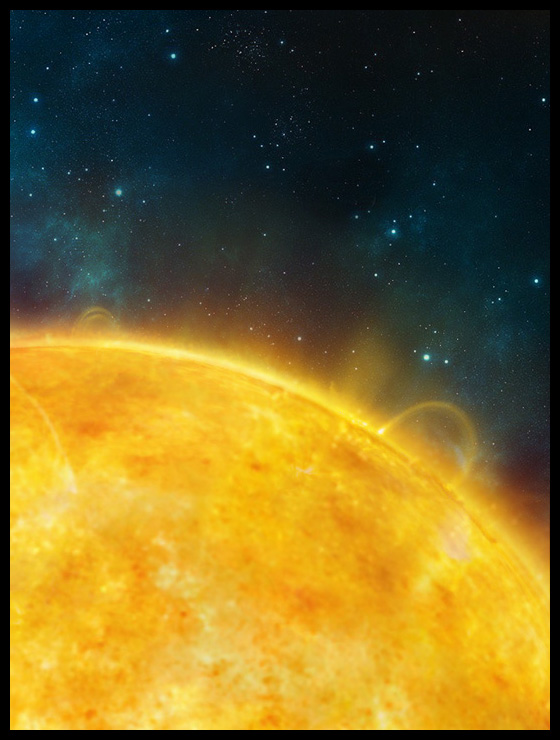
\includegraphics[width=\paperwidth]
    {awesome.jpg}}
\begin{frame}
    \titlepage{}
\end{frame}}%-------------------------------------------------------------%

\begin{frame}{Motivation/Main Scientific Question}
    {The coronal heating problem}
    \begin{itemize}
        \item ``Frozen-in'' magnetic field creates structure in the
            solar atmosphere, such as loops and prominences.
        \item Can observe oscillations and waves in the corona to extract
            properties about the solar photosphere and atmosphere.
            Phase speeds, amplitudes, dissipation, etc.\ can help determine
            physical properites that are otherwise inaccessible.
    \end{itemize}
\end{frame}%-------------------------------------------------------------%

\begin{frame}{Coronal seismology}{General idea}
    Based on how the \textcolor{arylyellow}{phase} speed is determined by
    local plasma parameters. Density structures act as waveguides,
    e.g.\ \textcolor{arylyellow}{coronal loops}.
    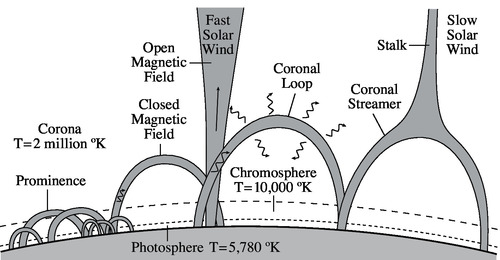
\includegraphics[width=\textwidth]{loop_diagram.jpg}
\end{frame}%-------------------------------------------------------------%

\begin{frame}{Modeling}{Theory before observations}
    \begin{columns}
        \column{0.6\textwidth}
        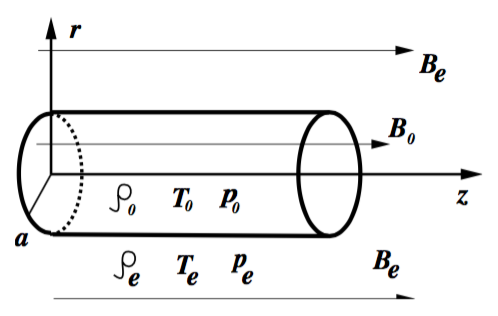
\includegraphics[width=\textwidth]{cylinder.png}
        \column{0.4\textwidth}
        \begin{itemize}
            \item Straight flux tube in uniform magnetic field.
            \item $ \xi(x) = \xi(r)e^{i(kz+m\phi)}  $
        \end{itemize}
    \end{columns}
\end{frame}%-------------------------------------------------------------%

\begin{frame}{Basic MHD}{What's the difference?}
    Characteristic speeds are determined by the environment
    (e.g.\ sounds waves traveling at $c_s=\sqrt{\frac{\gamma P}{\rho}}$
    Types of waves/oscillations:
    \begin{itemize*}
        \item Alfv\'en: $V_A = \frac{B}{\mu_0\rho}$
        \item Magnetoacoustic: $C_s = \sqrt{\frac{\gamma P}{\rho}}$
            \begin{itemize*}
                \item Fast $C_{A_0} < C_{fast} < C_{A_e} $
                \item Slow $C_{T_0} < C_{slow} < C_{s_0} $
            \end{itemize*}
    \end{itemize*}
\end{frame}%-------------------------------------------------------------%

\begin{frame}{Dispersion diagram}
    \begin{figure}
        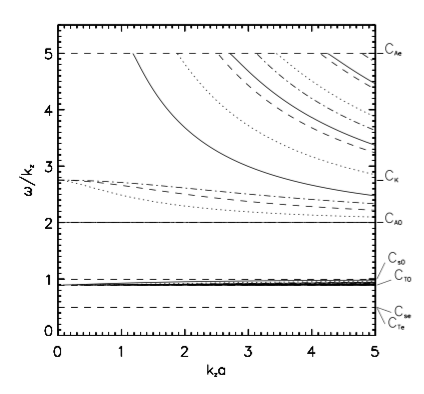
\includegraphics[width=3in]{disp_diagram.png}
    \end{figure}
\end{frame}%-------------------------------------------------------------%

\begin{frame}{Background}
    Nak, Asc, Roberts, all those common authors.
\end{frame}%-------------------------------------------------------------%

\begin{frame}{MHD modes}{Oscillations vs.\ waves}
    Or magnetoacoustic vs.\ Alfv\'en.
    Or fast vs.\ slow.
    \begin{itemize}
        \item Fast standing oscillations
            \begin{itemize}
                \item Kink
                \item Sausage
            \end{itemize}
        \item Slow standing oscillations
            \begin{itemize}
                \item Acoustic
            \end{itemize}
        \item Propagating slow waves
            \begin{itemize}
                \item Acoustic
            \end{itemize}
        \item Propagating fast waves
            \begin{itemize}
                \item Moreton
                \item EIT waves
            \end{itemize}
        \item Torsional modes (aka.\ Alfv\'en waves)
    \end{itemize}
\end{frame}%-------------------------------------------------------------%
\begin{frame}{Observational Methods}{How do you know what kind of mode
    you're looking at, or how to find potential MHD modes in the first place?}
    McIntosh et al.\ algorithm
\end{frame}%-------------------------------------------------------------%
\begin{frame}{Fast standing oscillations}{Kinks vs.\ Sausages}
%\begin{center}
\begin{columns}
        \column{0.6\textwidth}
    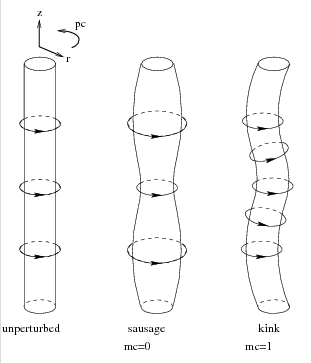
\includegraphics[width=2.5in]{kink_saus.png}
    %\par{\tiny image credit:\\
    %$https://inspirehep.net/record/1088737/files/figures_instab_locations.png$}
    %\end{center}
        \column{0.4\textwidth}
    \begin{block}{Kink}
        \begin{itemize}
            \item loop spatial displacement
            \item Asymmetric
            \item No intensity change
            \item $k\sigma \ll 1$, or $\sigma\ll\lambda$
        \end{itemize}
    \end{block}
    \begin{block}{Sausage}
        \begin{itemize}
            \item No loop spatial displacement
            \item Symmetric
            \item Intensity change\\ $\rightarrow$ density change
            \item $\lambda\sim\sigma$
        \end{itemize}
    \end{block}
\end{columns}
\end{frame}%-------------------------------------------------------------%
\begin{frame}{Fast standing oscillations}{Kinks vs.\ Sausages}
\begin{columns}
        \column{0.6\textwidth}
        The long-wavelength limit
        \column{0.4\textwidth}
    \begin{block}{Kink}
        \begin{itemize}
            \item $k\sigma \ll 1$, or $\sigma\ll\lambda$
        \end{itemize}
    \end{block}
    \begin{block}{Sausage}
        \begin{itemize}
            \item $\lambda\sim\sigma$
        \end{itemize}
    \end{block}
\end{columns}
\end{frame}%-------------------------------------------------------------%
\begin{frame}{Kink modes}{general characteristics}
    \begin{itemize}
        \item $c_k=\sqrt{\frac{\rho_oV_{Ao}^2 + \rho_cV_{Ac}^2}
            {\rho_o + \rho_c}}
            \approx V_A\sqrt{\frac{2}{1+\frac{\rho_e}{\rho_o}}} $
            in the low-$\beta$ plasma.
        \item $v_{ph} = \frac{\omega}{k} \approx C_k \gtrsim V_A $
        \item Period $P=\frac{2l}{V_A}\sqrt{\frac{1+\rho_e/\rho_o}{2}}$
            where $\lambda=2l$ ($l$ is the loop length).
            Typically, $l \approx 60-600$ Mm in the corona.
        \item ``current pinch'' instability
        \item Important observation from which magnetic field strength
            can be derived.
    \end{itemize}
\end{frame}%-------------------------------------------------------------%
\begin{frame}{Kink modes}
{Coronal loop oscillations observed with the
\emph{Transition Region And Coronal Explorer (TRACE)}}
    \begin{itemize}
        \item Not just a single, global mode.
        \item Gaussian vs.\ exponential
        \item Plasma motions around footpoints of coronal loops
    \end{itemize}
\end{frame}%-------------------------------------------------------------%
\begin{frame}{Kink modes}{``Excitation and damping of broadband kink waves
    in the solar corona''}
    Footpoint-driven, \emph{propagating} kink waves (which are
    temporally and spatially ubiquitous in the corona).
    Both standing and propagating kink waves are rapidly damped.
\end{frame}%-------------------------------------------------------------%
\begin{frame}{Sausage modes}{Observations of sausage modes in magnetic pores}
\end{frame}%-------------------------------------------------------------%
\begin{frame}{Sausage modes}{Sausage waves in transversely nonuniform
    monolithic coronal tubes}
\end{frame}%-------------------------------------------------------------%
\begin{frame}{Standing acoustic oscillations}
    Characteristics:
    \begin{itemize}
        \item Anisotropic (true in general for slow waves)
        \item Longitudinal/compressive
        \item Parallel to $\vec{B}$, perturbation of $\vec{B}$ is negligible.
        \item Pressure forces in opposition
        \item Impulsively excited
        \item Travel short distance (due to short decay time)
        \item Observed as variations in EUV emission intensity and Doppler shift
            (depending on orientation).
        \item Period = 7--31 minutes (20 minutes from another source)
        \item Decay times = 5.7--36.8 minutes
        \item Peak velocity = 200 km/sec
        \item Velocity and intensity are 90$^{\circ}$ out of phase.
    \end{itemize}
\end{frame}%-------------------------------------------------------------%
\begin{frame}{ac\_1}
\end{frame}%-------------------------------------------------------------%
\begin{frame}{ac\_2}
\end{frame}%-------------------------------------------------------------%
\begin{frame}{Propagating acoustic waves}
    Nodes are in motion; \emph{traveling waves}
    (Oscillations have fixed nodes).
\end{frame}%-------------------------------------------------------------%
\begin{frame}{pac\_1}
\end{frame}%-------------------------------------------------------------%
\begin{frame}{pac\_2}
\end{frame}%-------------------------------------------------------------%
\begin{frame}{Propagating fast waves}
    \begin{itemize}
        \item Moreton waves in the chromosphere
        \item Fast EUV waves in the corona
    \end{itemize}
\end{frame}%-------------------------------------------------------------%
\begin{frame}{pfw\_1}
\end{frame}%-------------------------------------------------------------%
\begin{frame}{pfw\_2}
\end{frame}%-------------------------------------------------------------%
\begin{frame}{Torsional modes}{aka.\ Alfv\'en wave}
\end{frame}%-------------------------------------------------------------%
\begin{frame}{tor\_1}
\end{frame}%-------------------------------------------------------------%
\begin{frame}{tor\_2}
\end{frame}%-------------------------------------------------------------%
\begin{frame}{Mixed modes}{Pulling individual modes out}
\end{frame}%-------------------------------------------------------------%
\begin{frame}{Important Properties}
    \begin{center}
        \begin{tabular}{c|c|c|c|}
            \cline{2-4} & \textbf{timescale} & \textbf{sizescale} &
                \textbf{obs.\ method}\\
            \hline \multicolumn{0}{|c|}{kink osc} & value & value & value\\
            \hline \multicolumn{0}{|c|}{sausage osc} & value & value & value\\
            \hline \multicolumn{0}{|c|}{acoustic osc} & value & value & value\\
            \hline \multicolumn{0}{|c|}{acoustic waves} & value & value & value\\
            \hline \multicolumn{0}{|c|}{fast waves} & value & value & value\\
            \hline \multicolumn{0}{|c|}{torsional modes} & value & value & value\\
            \hline \multicolumn{0}{|c|}{mixed modes} & value & value & value\\
            \hline
        \end{tabular}
    \end{center}
\end{frame}%-------------------------------------------------------------%
\begin{frame}{Example Table}
\begin{center}
   \begin{tabular}{cc|c|c|}
% row 1
   \cline{3-4} & & \multicolumn{2}{|c|}{Condition (Gold standard)}\\
% row 2
   \cline{3-4} & & True & False \\
   \hline
% row 3 (and 4) - multirow
   \multicolumn{1}{|c|} % add in vertical lines
   {\multirow{2}{*}{Test outcome}}& % Text covers rows 3 and 4
 % row 3
   \multicolumn{1}{|c|}{Positive} %
     & True Positive \cellcolor{green} & False Positive\cellcolor{red}\\
 % row 4
   \cline{2-4} \multicolumn{1}{|c|}{}
     & \multicolumn{1}{|c|}{Negative}
     & False Negative\cellcolor{red} & True Negative \cellcolor{green}\\
    \hline
    \end{tabular}
\end{center}
\end{frame}%-------------------------------------------------------------%

\begin{frame}{Example of Two Column Output}
    \begin{columns}[c]
        \column{1.5in}
            Practical \TeX\ 2005\\
            Practical \TeX\ 2005\\
            Practical \TeX\ 2005
        \column{1.5in}
            % put nice little frame around graphic
            \framebox{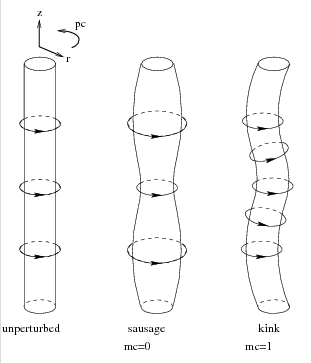
\includegraphics[width=1.5in]{kink_saus.png}}
    \end{columns}
\end{frame}%-------------------------------------------------------------%


\begin{frame}{My Research}
\end{frame}%-------------------------------------------------------------%

\end{document}
